\begin{task}
\TT{Wyznacz współczynniki zespolonego szeregu Fouriera dla okresowego sygnału $g(t)$ przedstawionego na rysunku. Wykorzystaj własności szeregu Fouriera oraz współczynniki zespolonego szeregu Fouriera wyznaczone w zadaniu \ref{TaskKW010}}{Calculate coefficients of the periodic signal $f(t)$ shown below for the expansion into a complex exponential Fourier series. Draw magnitude and phase spectra.}


\begin{figure}[H]
  \centering
  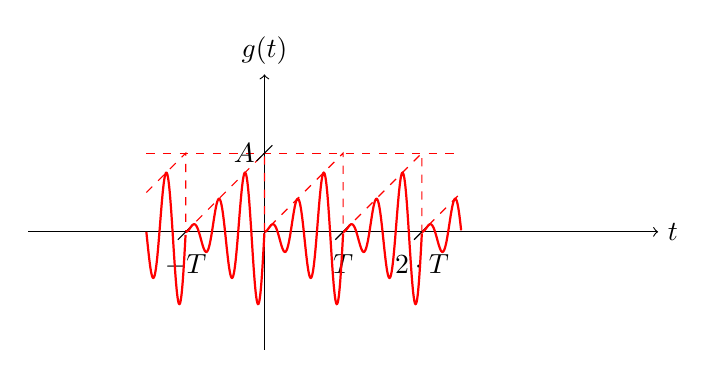
\begin{tikzpicture}
  %\draw (0,0) circle (1in);
  \draw[->] (-3.0,+0.0) -- (+5.0,+0.0) node[right] {$t$};
  \draw[->] (+0.0,-1.5) -- (+0.0,+2.0) node[above] {$g(t)$};
  \draw[-,red, dashed] (-1.5,0.5) -- (-1.0,1.0) -- (-1.0,0.0) -- (0.0,1.0) -- (0.0,+0.0) -- (+1.0,+1.0) -- (1.0,+1.0) -- (+1.0,+0.0) -- (1.0,+0.0) -- (+2.0,+1.0) -- (+2.0,+0.0) -- (2.5,0.5);
  \draw[-,red, dashed] (-1.5,1.0) -- (2.5,1.0);
  %\draw[-] (-1.0-0.1,-0.1)--(-1.0+0.1,0.1) node[midway, below, outer sep=10pt,align=center] {$-\frac{T}{2}$};
  \draw[-] (-1.0-0.1,-0.1)--(-1.0+0.1,0.1) node[midway, below, outer sep=5pt] {$-T$};
  \draw[-] (+1.0-0.1,-0.1)--(+1.0+0.1,0.1) node[midway, below, outer sep=5pt] {$T$};
  \draw[-] (+2.0-0.1,-0.1)--(+2.0+0.1,0.1) node[midway, below, outer sep=5pt] {$2 \cdot T$};
  \draw[-] (-0.1,+1.0-0.1)--(+0.1,+1.0+0.1) node[midway, left] {$A$};
  
  \draw[scale=1.0,domain=0:1.0,samples=200,smooth,variable=\x,red,thick] plot ({\x},{0.0+\x*sin(\x*180.0/3.141592*6*3.141592/1.0)});
  
  \draw[scale=1.0,domain=1.0:2.0,samples=200,smooth,variable=\x,red,thick] plot ({\x},{0.0+(\x-1.0)*sin(\x*180.0/3.141592*6*3.141592/1.0)});
  
  \draw[scale=1.0,domain=-1.0:0.0,samples=200,smooth,variable=\x,red,thick] plot ({\x},{0.0+(\x+1.0)*sin(\x*180.0/3.141592*6*3.141592/1.0)});
  
  \draw[scale=1.0,domain=2.0:2.5,samples=200,smooth,variable=\x,red,thick] plot ({\x},{0.0+(\x-2.0)*sin(\x*180.0/3.141592*6*3.141592/1.0)});
  
  \draw[scale=1.0,domain=-1.5:-1.0,samples=200,smooth,variable=\x,red,thick] plot ({\x},{0.0+(\x+2.0)*sin(\x*180.0/3.141592*6*3.141592/1.0)});
  
  \end{tikzpicture}
\end{figure}

% To be done

\TT{W pierwszej kolejności należy opisać sygnał w pierwszym okresie za pomocą wzoru.}{Periodic signal $f(t)$, as a piecewise linear function, is given by:}

\begin{equation}
   g(x)=\frac{A}{T}\cdot t \cdot sin\left(\frac{6\pi}{T}\cdot t\right)
\end{equation}

\TT{Można zauważyć iż sygnał $g(t)$ jest z modulowaną wersją sygnału $f(t)$ z zadania \ref{TaskKW010}}{}
\begin{align*}
g(t) &= f\left(t\right) \cdot sin\left(\frac{6\pi}{T}\cdot t\right) \\
&=\left\{\begin{array}{ll}
\EulerSin
\end{array}\right\}=\\
&= f\left(t\right) \cdot \frac{e^{\jmath \cdot \frac{6\pi}{T}\cdot t} - e^{-\jmath \cdot \frac{6\pi}{T}\cdot t}}{2 \cdot \jmath} \\
&= \frac{1}{2\cdot \jmath} \left( f\left(t\right) \cdot e^{\jmath \cdot \frac{6\pi}{T}\cdot t} - f\left(t\right) \cdot e^{-\jmath \cdot \frac{6\pi}{T}\cdot t}\right)
\end{align*}

\TT{Współczynniki trygonometrycznego szeregu Fouriera $a_k$ i $b_k$ dla sygnału $f(t)$ wyznaczone w zadaniu \ref{TaskKW010} wynoszą:}{}
\begin{align*}
a_0&=\frac{A}{2}\\
a_k&=0\\
b_k&=-\frac{A}{k\cdot \pi}\\
\end{align*}

\TT{Korzystając z zależności miedzy współczynnikami $F_k$ zespolonego szeregu Fouriera i współczynnikami $a_k$ i $b_k$ trygonometrycznego szeregu Fourier możemy wyznaczyć współczynniki $F_k$ zespolonego szeregu Fouiera}{xx}

\begin{align*}
F_0 &= a_0\\
F_k &= a_k - \jmath \cdot b_k
\end{align*}

\TT{a wiec dla sygnału $f(t)$ z zadania \ref{TaskKW010} współczynniki zespolonego szeregu Fouriera wynoszą:}{xx}

\begin{align*}
F_0 &= a_0 = \frac{A}{2}\\
F_k &= a_k - \jmath \cdot b_k=\\
& = 0 - \jmath \cdot \left(-\frac{A}{k\cdot \pi}\right)=\\
& = \jmath \cdot \frac{A}{k\cdot \pi}\\
\end{align*}

\TT{Korzystając z twierdzenia o modulacji można wyznaczyć współczynniki $G_k$ na podstawie współczynników $F_k$ sygnału $f(t)$ jako:}{}
\begin{align*}
g^1(t) &= f(t)\cdot e^{\jmath \cdot \frac{2\pi}{T}\cdot k_0 \cdot t}\\
G^1_k &= F_{k-k_0}
\end{align*}

\TT{W przypadku analizowanego sygnału twierdzenie o modulacji należy zastosować dwa razy}{}

\begin{align*}
g(t) &= \frac{1}{2\cdot \jmath} f(t)\cdot e^{\jmath \cdot \frac{2\pi}{T}\cdot k^1_0 \cdot t} - \frac{1}{2\cdot \jmath} f(t)\cdot e^{\jmath \cdot \frac{2\pi}{T}\cdot k^2_0 \cdot t}\\
g(t) & = g^1(t) - g^2(t)\\
G_k &= G^1_k - G^2_k\\
G_k &= \frac{1}{2\cdot \jmath} \left( F_{k-k^1_0} - F_{k-k^2_0} \right)
\end{align*}
  
\TT{W obu przypadkach funkcja $f(t)$ mnożona jest przez czynnik $e^{\jmath \cdot \frac{6\pi}{T}\cdot t}$ (z uwzględnieniem zmiany znaku). Z tego czynnika można wydzielić wartość $k^1_0$ i $k^2_0$.}{}

\begin{align*}
e^{\jmath \cdot \frac{6\pi}{T}\cdot t} &= e^{\jmath \cdot \frac{2 \ cdot 3\pi}{T}\cdot t}\\
&=e^{\jmath \cdot \frac{2\pi}{T} \cdot 3\cdot t} \Rightarrow k^1_0 = 3\\
\end{align*}

\begin{align*}
e^{-\jmath \cdot \frac{6\pi}{T}\cdot t} &= e^{-\jmath \cdot \frac{2 \ cdot 3\pi}{T}\cdot t}\\
&=e^{-\jmath \cdot \frac{2\pi}{T} \cdot 3\cdot t} \\
&=e^{\jmath \cdot \frac{2\pi}{T} \cdot \left(-3\right) \cdot t} \Rightarrow k^2_0 = -3\\
\end{align*}
  
\TT{Wstawiając wartości współczynników $F_k$ otrzymujemy}{}
\begin{align*}
G_k &= \frac{1}{2\cdot \jmath} \left( F_{k-k^1_0} - F_{k-k^2_0} \right) =\\
 &= \frac{1}{2\cdot \jmath} \left( 
\jmath \cdot \frac{A}{\left(k-k^1_0\right) \cdot \pi}
 - \jmath \cdot \frac{A}{\left(k-k^2_0\right)\cdot \pi} \right) = \\
&=\left\{\begin{array}{ll}
k^1_0 = 3 & k^2_0 = -3
\end{array}\right\}=\\ 
&= \frac{1}{2\cdot \jmath} \left( 
\jmath \cdot \frac{A}{\left(k-3\right) \cdot \pi}
- \jmath \cdot \frac{A}{\left(k-\left(-3\right)\right)\cdot \pi} \right) = \\
&= \frac{1}{2\cdot \jmath} \cdot \jmath \cdot \frac{A}{\pi}\left( 
\frac{1}{k-3}
- \frac{1}{k+3} \right) = \\
&= \frac{1}{2} \cdot \frac{A}{\pi}\left( 
\frac{k+3}{\left(k-3\right)\cdot \left(k+3\right)}
- \frac{k-3}{\left(k+3\right)\cdot \left(k-1\right)} \right) = \\
&= \frac{1}{2} \cdot \frac{A}{\pi}\cdot 
\frac{k+3-\left(k-3\right)}{\left(k-3\right)\cdot \left(k+3\right)} = \\
&= \frac{1}{2} \cdot \frac{A}{\pi}\cdot 
\frac{k+3-k+3}{k^2-9} = \\
&= \frac{1}{2} \cdot \frac{A}{\pi}\cdot 
\frac{6}{k^2-9} = \\
&= \frac{A}{\pi}\cdot 
\frac{3}{k^2-9}\\
\end{align*}

\TT{A wiec współczynniki $G_k$ dla sygnału $g(t)$ są równe $\frac{A}{\pi}\cdot 
  \frac{3}{k^2-9}$, dla $k \neq 3 \wedge k\neq -3$. Oznacza to iż współczynnik dla $k=3$ i $k=-3$ musimy wyznaczyć jeszcze raz analizując dokładnie co podstawiamy. Zacznijmy od wyznaczenia $G_3$ }{}

\begin{align*}
G_3 &= \frac{1}{2\cdot \jmath} \left( F_{3-k^1_0} - F_{3-k^2_0} \right) = \\
&=\left\{\begin{array}{ll}
k^1_0 = 3 & k^2_0 = -3
\end{array}\right\}=\\ 
&= \frac{1}{2\cdot \jmath} \left( F_{3-3} - F_{3-\left(-3\right)} \right) =\\
&= \frac{1}{2\cdot \jmath} \left( F_{0} - F_{3+3} \right) =\\
&= \frac{1}{2\cdot \jmath} \left( F_{0} - F_{6} \right)
\end{align*}

\TT{A wiec musimy podstawić wartość współczynników $F_0$ oraz $F_{6}$}{}

\begin{align*}
G_3 &= \frac{1}{2\cdot \jmath} \left( F_{0} - F_{6} \right) =\\
&= \frac{1}{2\cdot \jmath} \left(\frac{A}{2} - \jmath \cdot \frac{A}{6\cdot \pi}\right) = \\
&= \frac{A}{4\cdot \jmath} - \frac{A}{2\cdot 6\cdot \pi} = \\
&= \frac{A}{4\cdot \jmath} - \frac{A}{12 \cdot \pi}=\\
&= - \frac{A}{12 \cdot \pi} + \frac{A}{4\cdot \jmath}\\
\end{align*}


\TT{Podobnie wyznaczymy współczynnik $G_{-3}$ }{}

\begin{align*}
G_{-3} &= \frac{1}{2\cdot \jmath} \left( F_{-3-k^1_0} - F_{-3-k^2_0} \right) = \\
&=\left\{\begin{array}{ll}
k^1_0 = 3 & k^2_0 = -3
\end{array}\right\}=\\ 
&= \frac{1}{2\cdot \jmath} \left( F_{-3-3} - F_{-3-\left(-3\right)} \right) =\\
&= \frac{1}{2\cdot \jmath} \left( F_{-6} - F_{-3+3} \right) =\\
&= \frac{1}{2\cdot \jmath} \left( F_{-6} - F_{0} \right)
\end{align*}

\TT{A wiec musimy podstawić wartość współczynników $F_{-6}$ oraz $F_{0}$}{}

\begin{align*}
G_3 &= \frac{1}{2\cdot \jmath} \left( F_{-6} - F_{0)} \right) =\\
&= \frac{1}{2\cdot \jmath} \left( \jmath \cdot \frac{A}{-6 \cdot\pi} - \frac{A}{2}\right) = \\
&= \frac{A}{-12 \cdot\pi} - \frac{A}{4 \cdot \jmath} = \\
&= -\frac{A}{12 \cdot\pi} - \frac{A}{4 \cdot \jmath}\\
\end{align*}

\TT{Można także zauważyć iż nie ma konieczności wyznaczania osobno wartości współczynnika dla $k=0$, ponieważ można go wyznaczyć z ogólnego wzoru na $G_k$.}{}


\TT{Ostatecznie współczynniki zespolonego szeregu Fouriera dla funkcji przedstawionej na rysunku przyjmują wartości.}{To sum up, coefficients for the expansion into a complex exponential Fourier series are given by:}
\begin{align*}
G_{-3}&=-\frac{A}{12 \cdot\pi} + \frac{A}{4 \cdot \jmath}\\
G_{3}&=-\frac{A}{12 \cdot\pi} - \frac{A}{4 \cdot \jmath}\\
G_k&=\frac{A}{\pi}\cdot 
\frac{3}{k^2-9}
\end{align*}

\end{task}